
\chapter{Primeros pasos con Function v0.5}
   En este capitulo se echa un vistazo rápido a las características y usos del software Function v0.5.
   
   \section{¿Qué es Function v0.5?}
      Function v0.5 es un software para evaluación de expresiones matemáticas, programación de funciones y algoritmos de manera sencilla y elegante con un lenguaje construido sobre una variante extendida de las expresiones lambda.% ademas Function v0.5 es software---.
      
   \section{Descarga e instalación}
   
   \section{La interfaz}
      Al ejecutar Function v0.5 se despliega la consola de comandos (o {\it shell} en ingles), en esta aparece un puntero representado por ``\arrowprompter'' desde el cual podemos ingresar el código a ser interpretado una vez que presionemos la tecla {\it RETURN}, tales códigos pueden ser evaluar una expresion, construir una nueva función, controlar el sistema, etc. 
   
      \begin{figure}[htbp]
         \caption{Interfaz gráfica}\label{fg:console}
         \begin{center}
            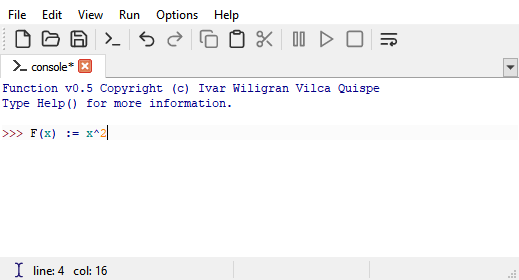
\includegraphics[scale=2.5]{FunctionImg1.png}
         \end{center}   
      \end{figure}
      
      Por ejemplo escribamos \texttt{35 + 12\^{}(1/2) - 4*Sin(-1.45)} después del puntero y ahora presionemos la tecla {\it RETURN}:
      
      \begin{fxcode}
         \arrowcode{35 + 12\^{}(1/2) - 4*Sin(-1.45)}\\
         \outcode{42.4349535792881} \codecomment{el resultado de sumar $2 + 3$}
      \end{fxcode}
      
      Esta es el resultado de evaluar la expresion $35 + 12^{1/2} - 4*\sin(-1.45)$
   
   \section{El lenguaje}
      Function v0.5 interpreta comandos que es un código que representa un bloque básico de ejecución, en total son 8 clases de comandos:
      
      \begin{longtable}[c]{ll}
         \caption{Lista de comandos}\label{tb:cmds} \\ \hline
         {\bf Nombre}      & {\bf Ejemplo} \\ \hline
         Ejecutar guiones  & \texttt{run "lib\textbackslash\textbackslash prelude.fx"} \\
         Notaciones        & \texttt{infixl 175 +} \\
         Sinónimo de tipo  & \texttt{String ::= [char]} \\
         Tipado heredable  & \texttt{f :: real -> real} \\
         Definiciones      & \texttt{f(x) := x\^{}2 + 2*x - 1} \\
         Asignaciones      & \texttt{x <- [[1, 0], [0, 1]]} \\
         Limpieza          & \texttt{clear f} \\
         Evaluación        & \texttt{2 + 3*x} \\
      \end{longtable}
      
      Ejecutar un guion significa interpretar todos los comandos escritos en un archivo de texto que contiene código Function v0.5 este archivo es llamado guion (o {\it script} en ingles).
      
      \begin{fxcode}
         \arrowcode{run "lib\textbackslash\textbackslash acme\textbackslash\textbackslash emptyscript.fx"}
      \end{fxcode}
      
      Los guiones suelen tener por defecto la extensión ``.fx''.
      
      Una definición se puede hacer directamente escribiendo una función con su respectiva expresion de retorno.
      
      \begin{fxcode}
         \arrowcode{f(x) := x\^{}3 + x - 3}
      \end{fxcode}
      
      Las asignaciones evalúan una expresión y la asignan a una variable o identificador pero sin mostrar el resultado.
      
      \begin{fxcode}
         \arrowcode{v <- 12*2 - 1}
      \end{fxcode}
      
      Para saber el valor de la variable se puede proceder a evaluarla:
      
      \begin{fxcode}
         \arrowcode{v}\\
         \outcode{23}
      \end{fxcode}
      
      La evaluación de expresiones es un comando que evalúa una expresión y luego muestra su resultado.
      
      \begin{fxcode}
         \arrowcode{23 + 4*5 - 2*(7 + 1)/(3\^{}4) + (-4)}\\
         \outcode{38.8024691358025}
      \end{fxcode}
      
      Para conocer nuevamente el valor de la evaluación anterior se puede utilizar la función \texttt{Ans()}.
      
      \begin{fxcode}
         \arrowcode{Ans()}\\
         \outcode{38.8024691358025}
      \end{fxcode}
      
      El valor de esta función cambia cada vez que se ejecute un comando de evaluación.
      
      Algunas de las funciones y operadores en Function v0.5 son:
      
      \begin{longtable}[c]{|l|c|l|l|l|}
         \caption{Funciones y operadores básicos}\label{tb:basicopr} \\ \hline
         {\bf Nombre}           & {\bf Símbolo} & {\bf Ejemplo} & {\bf Resultado}  & {\bf Descripción}\\ \hline
         suma           & \texttt{+} & \texttt{3 + 4} & \texttt{7}  & suma de números reales\\ \hline
         resta          & \texttt{-} & \texttt{4 - 1} & \texttt{3}  & resta de números reales\\ \hline
         multiplicación & \texttt{*} & \texttt{5 * 5} & \texttt{25}  & multiplicación de números reales\\ \hline
         división       & \texttt{/} & \texttt{4 / 16} & \texttt{0.25}  & División de números reales\\ \hline
         potenciación   & \texttt{\^} & \texttt{4~\^~0.5} & \texttt{2}  & Potenciación de números reales\\ \hline
         negación   & \texttt{-} & \texttt{- 3.56} & \texttt{-3.56}  & el negativo de un número\\ \hline
         seno & \texttt{Sin} & \texttt{Sin(0.7512)} & \texttt{0.6825162} & La función seno \\ \hline
         coseno & \texttt{Cos} & \texttt{Cos(0.7512)} & \texttt{0.730870} & La función coseno \\ \hline
         tangente & \texttt{Tan} & \texttt{Tan(0.7512)} & \texttt{0.933840} & La función tangente \\ \hline
         arco seno & \texttt{ASin} & \texttt{ASin(0.7512)} & \texttt{0.8498781} & La función arco seno \\ \hline
         arco coseno & \texttt{ACos} & \texttt{ACos(0.7512)} & \texttt{0.7209181} & La función arco coseno \\ \hline
         arco tangente & \texttt{ATan} & \texttt{ATan(0.7512)} & \texttt{0.6442686} & La función arco tangente \\ \hline
      \end{longtable}
      
      Se pueden utilizar los tabuladores para crear espacios mas rápidamente, estos tabuladores tienen un tamaño equivalente a 8 espacios en blanco.
      
   \section{Control del sistema}
      Para realizar algunas órdenes para el sistema como por ejemplo cerrar el software se pueden recurrir a las funciones siguientes que ademas de devolver un valor realiza una acción.
      
      \begin{longtable}[c]{|l|l|l|}
         \caption{Ordenes básicas}\label{tb:basicord} \\ \hline
         {\bf Nombre} & {\bf Representación} & {\bf Descripción}\\ \hline
         respuesta    & \texttt{Ans()} & devuelve el resultado de la expresion anterior evaluada\\ \hline
         ayuda    & \texttt{Help()} & despliega la ayuda básica de Function v0.5\\ \hline
         reiniciar & \texttt{Restart()} & reinicia el sistema\\ \hline
         interrumpir    & \texttt{Interrupt()} & interrumpe una tarea llevada a cabo por Function v0.5\\ \hline
         salir    & \texttt{Quit()} & finaliza el sistema y cierra el programa\\ \hline
      \end{longtable}
      
      \begin{fxcode}
         \arrowcode{Ans()}\codecomment{resultado}
      \end{fxcode}
      
      \begin{fxcode}
         \arrowcode{Help()}\codecomment{ayuda}
      \end{fxcode}
      
      \begin{fxcode}
         \arrowcode{Restart()}\codecomment{reiniciar}
      \end{fxcode}
      
      \begin{fxcode}
         \arrowcode{Interrupt()}\codecomment{interrumpir}
      \end{fxcode}
      
      \begin{fxcode}
         \arrowcode{Quit()}\codecomment{salir}
      \end{fxcode}
      
      Similar a la función del sistema \texttt{Interrupt()} existe un atajo para cuando la ejecución de un comando se hace demasiado largo se pueda abortar su ejecución, esto se consigue presionando la combinación de teclas {\it Ctrl+BREAK} que interrumpe la ejecución y vuelve a mostrar el puntero.
      \\
      
      Por ultimo si se ingresa un carácter no reconocido o le falta algún argumento a los operadores, el sistema Function v0.5 detecta dicho error y lanza un mensaje indicando nuestro error.
      
      \begin{fxcode}
         \arrowcode{¿}\\
         \outcode{ERROR - lexical error in command 1 line 1, unexpected input "¿"}
      \end{fxcode}
      
      \begin{fxcode}
         \arrowcode{2 + }\\
         \outcode{ERROR - syntax error in command 1 line 1, missing right argument for "\texttt{+}"}
      \end{fxcode}
      
   
   
   
   
   
   
   
   
   
   
   
   